\documentclass{article}
\usepackage{graphicx}
\usepackage{color}
\usepackage{amssymb}
\usepackage{amsmath}
\usepackage{multirow}
\usepackage{multicol}
\usepackage{array}
\usepackage{rotating,capt-of}
\usepackage[small]{caption}
\usepackage{booktabs}
%\usepackage{float} % for placing figures where i want
\usepackage{afterpage}
\usepackage{epsfig, a4wide}

\usepackage{tikz,graphicx}
\usetikzlibrary{shapes.geometric, arrows}
\usetikzlibrary{shapes.misc, positioning}
\usetikzlibrary{backgrounds}

\definecolor{lavander}{cmyk}{0,0.48,0,0}
\definecolor{violet}{cmyk}{0.79,0.88,0,0}
\definecolor{burntorange}{cmyk}{0,0.52,1,0}

\def\lav{lavander!90}
\def\oran{orange!30}

\tikzstyle{neighbors}=[draw,circle,violet,bottom color=\lav,
                  top color= white, font=\scriptsize,text=violet,minimum width=10pt]
\tikzstyle{queries}=[draw,circle,burntorange, left color=\oran,
                       text=violet,minimum width=30pt]

\tikzstyle{io} = [trapezium, trapezium left angle=70, trapezium right angle=110, minimum width=3cm, minimum height=1cm, text centered, draw=black, color=burntorange,left color=\oran,text=black,font=\Large]

\tikzstyle{res} = [trapezium, trapezium left angle=70, trapezium right angle=110, minimum width=3cm, minimum height=1cm, text centered, draw=black, color=violet,bottom color=\lav, top color=white,text=black,font=\Large]

\tikzstyle{process} = [rectangle, minimum width=3cm, minimum height=1cm, text centered, draw=violet, bottom color=\lav, top color=white,font=\Large]

\tikzstyle{grey} = [ rectangle, rounded corners=10pt, bottom color=black!10, top color=black!2,font=\Large]

\tikzstyle{aro} = [->, thick,  shorten >=2pt, shorten <=2pt]



\newcommand{\myparagraph}[1]{
  \paragraph*{\normalfont\itshape #1}\hspace{5pt}}

% strange snos
\definecolor{purple}{RGB}{180,90,200}
\definecolor{dgreen}{RGB}{0,160,0}
\definecolor{turquoise}{RGB}{0,180,140}
\renewcommand\dblfloatpagefraction{0.03}
\renewcommand\topfraction{.95}
\renewcommand\bottomfraction{.95}
\renewcommand\textfraction{.05}
\renewcommand\floatpagefraction{.95}
\renewcommand\dbltopfraction{.95}
\renewcommand\dblfloatpagefraction{.95}
\newcommand{\TODO}[1] {\begingroup\color{red}#1\endgroup}
\newcommand{\SC}[1] {\begingroup\color{purple}#1\endgroup}
\newcommand{\ACC}[1]{\emph{\textbf{#1}}}
\newcommand{\s}[1]{\begin{tiny}#1\end{tiny}}
\newcommand{\url}[1]{\texttt{http://\small #1}}
\newcommand{\maxentscan}{\texttt{MaxEntScan}}
\newcommand{\NEW}[1]{\begingroup\color{black}#1\endgroup}

%% programs
\newcommand{\spps}{\texttt{SPPS}}
\newcommand{\tri}{\texttt{TRI\_tool}}
\newcommand{\lr}{\texttt{LR\_PPI}}

%% databases
\newcommand{\ncbi}{\texttt{NCBI}}
\newcommand{\nega}{\texttt{Negatome Database}}
\newcommand{\kups}{\texttt{KUPS}}

%\newcommand{\tool}{\texttt{rfPRO}}
%\newcommand{\tool}{\texttt{jackProt}}
\newcommand{\tool}{\texttt{ProteinPrompt}}
\newcommand{\website}{\url{proteinformatics.org/\tool}}

\newcommand{\Hsa}{\emph{Homo sapiens}}
\newcommand{\hsa}{\emph{H.sapiens}}

%\journal{Nature}

\bibliographystyle{naturemag}
\title{\tool: fast and accurate prediction of Protein-Protein-Interactions}

\author{ Sebastian Canzler$^{1,3}$, Ren\'{e} Staritzbichler$^{2,3}$}


\begin{document}

\maketitle





\begin{abstract}

 Proteins are the 'machines' of the cell, consisting of linear chains of amino acids.
They fulfil manyfold roles as receptors, enzymes, transporters or molecular factories.
Understanding biological processes often depends on insight into the interaction between proteins.

Computations of the binding behaviour of proteins can both complement and guide experimental studies.
However, calculating protein binding in atomic detail is highly time consuming and requires  knowledge about their structures.
While proteins are complex threedimensional molecules, their structure, function and also binding behaviour is encoded in their amino acid sequence.
In turn, many of their properties and behaviour can be understood from their sequence.
We developed \tool, a tool based on machine learning, using the sequences of protein pairs as input to estimate their tendency to bind.

Starting point of the training of a learning algorithm, was the collection of a comprehensive dataset from basically all available sources.
Positive data was collected from the
Database of Human Interacting Proteins (DIP)
\cite{Salwinski:2004},
Human Protein Reference Database (HPRD)
\cite{Keshava_Prasad:2009},
Protein  Database (PDB) \cite{Berman:2000}.
We also included annotations retrieved from the
KUPS server \cite{Chen:2011}.
Negative data was collected
from the Negatome Database \cite{Blohm:2014}  and the KUPS server.


After collecting such a broad database, a thorough curation was imperative.
We performed several iterations of filtering and cleanup, automated in terms of computational tools, as well as through manual inspection.

Obviously, the quality of a learning method depends crucially both on the amount as well as on the quality of the datasets used for training.
But the key to 'stellar' performance lays often in the way, the data is presented to the learning algorithm itself. 
Sequences can not be fed into learning algorithms directly, but need to be translated into descriptors that enable the learning algorithm to spot the patterns, whether a pair of sequences will bind or not.
We identified autocorralation profiles on hydrophobicity scales to best capture the binding propensity. 

Learning algorithms themselves are available in many implementations.
Most prominently in the rise of learning approaches in biology  are artificial neural networks (ANN).
We compared ANNs with support vector machines and several other learning methods.
As a result, we identified the random forrest approach as leading to the cleanest separation of binders and non-binders.

The described procedure resulted in an accurracy far above any other available tool, with the following values:
area under curve of 0.94,
specificity of 0.88
sensitivity: 0.84,
and a total accurracy of 0.86.
Testing was performed on a challenging dataset, as the comparison with other tools shows (see Fig. \ref{fig:comparison}).

\tool\  is available online, free for academic users. The server allows users to scan several databases for potential binders of their query sequence. 
Scanning a query sequence against the human database requires around one minute. 
(The URL will be ready for testing by the time of submission of the full draft.) \\
\noindent \centerline{\website.} \\

\end{abstract}



\begin{figure}
  \centerline{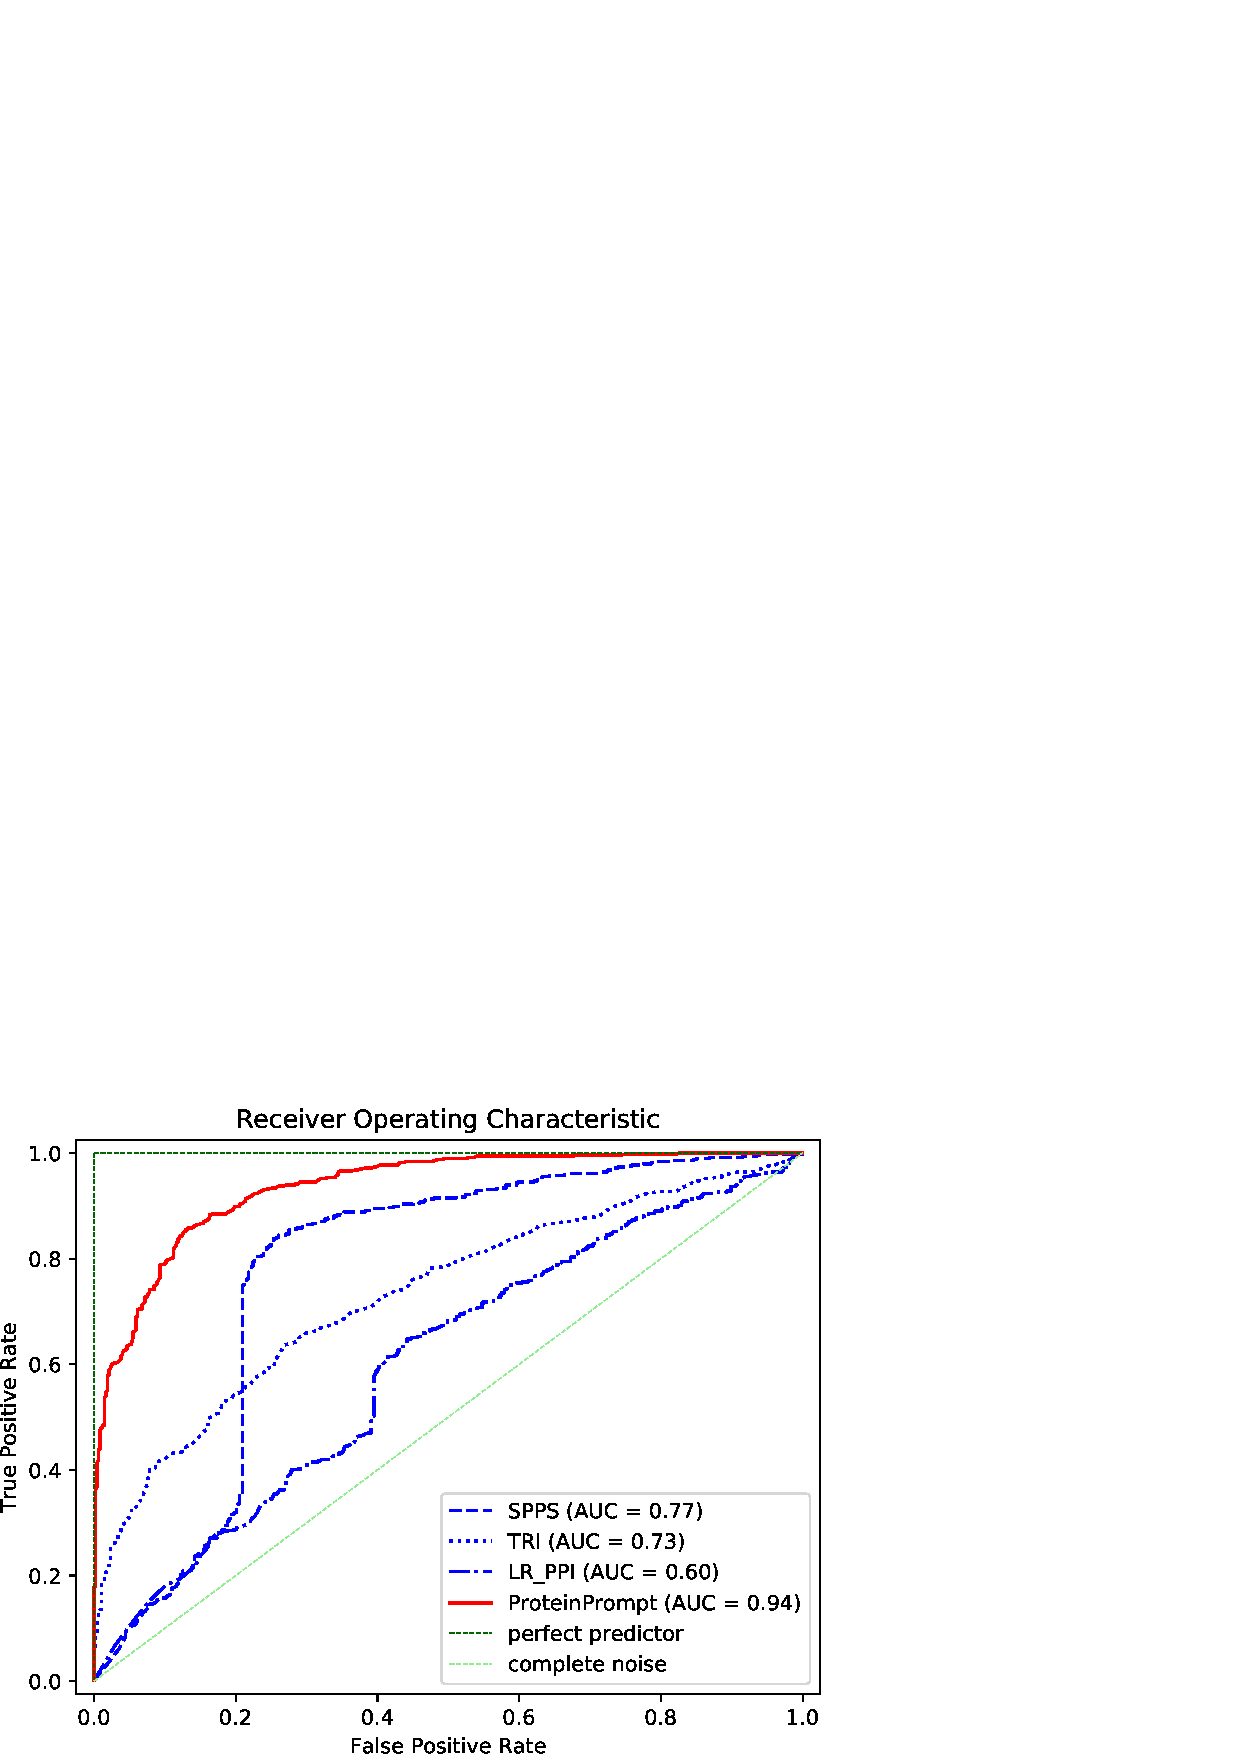
\includegraphics[width=0.5\textwidth]{img/comparison_roc.pdf}}
  \caption{Quality estimate: comparison of ROC-curves between \tool, \spps, \tri, \lr\ using a diminished test dataset including 968 protein-protein pairs.}
  \label{fig:comparison}
\end{figure}


\begin{figure}
  \iffalse
%\documentclass{article}
%\usepackage{tikz}
%\usetikzlibrary{shapes.geometric, arrows}
%\usetikzlibrary{shapes.misc, positioning}
%
%\definecolor{lavander}{cmyk}{0,0.48,0,0}
%\definecolor{violet}{cmyk}{0.79,0.88,0,0}
%\definecolor{burntorange}{cmyk}{0,0.52,1,0}
%
%\def\lav{lavander!90}
%\def\oran{orange!30}
%
%\tikzstyle{neighbors}=[draw,circle,violet,bottom color=\lav,
%                  top color= white, font=\scriptsize,text=violet,minimum width=10pt]
%\tikzstyle{queries}=[draw,circle,burntorange, left color=\oran,
%                       text=violet,minimum width=30pt]
%
%\tikzstyle{io} = [trapezium, trapezium left angle=70, trapezium right angle=110, minimum width=3cm, minimum height=1cm, text centered, draw=black, color=burntorange,left color=\oran,text=black]
%
%\tikzstyle{res} = [trapezium, trapezium left angle=70, trapezium right angle=110, minimum width=3cm, minimum height=1cm, text centered, draw=black, color=violet,bottom color=\lav, top color=white,text=black]
%
%\tikzstyle{process} = [rectangle, minimum width=3cm, minimum height=1cm, text centered, draw=violet, bottom color=\lav, top color=white]
%
%\tikzstyle{grey} = [ rectangle, rounded corners=10pt, bottom color=black!10, top color=black!2] 
%
%\tikzstyle{aro} = [->, thick,  shorten >=2pt, shorten <=2pt]
%
%\begin{document}
\fi

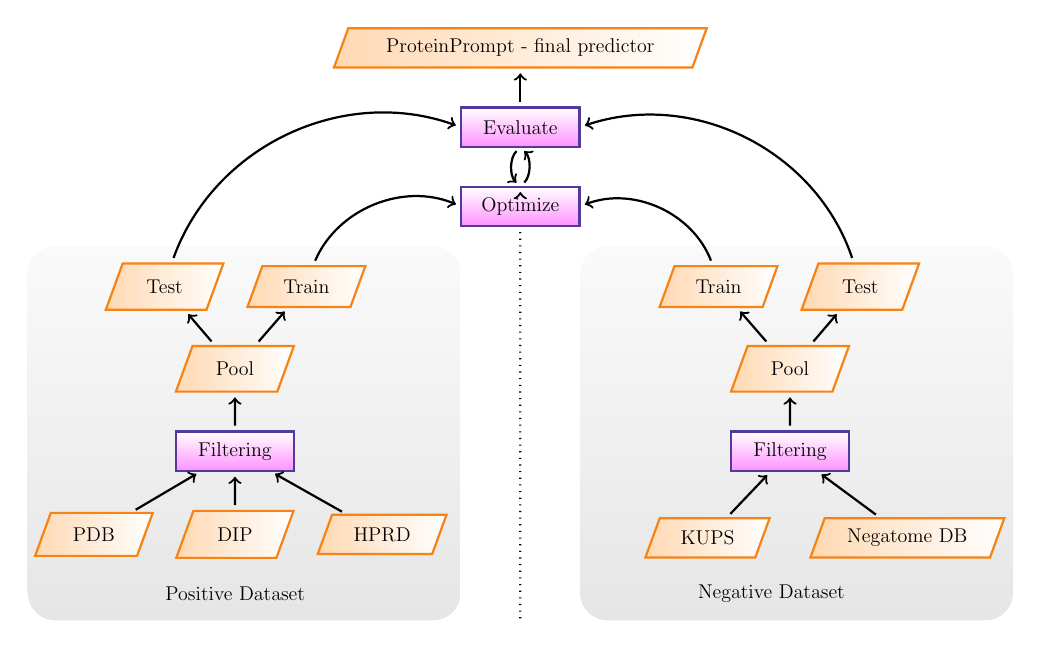
\begin{tikzpicture}[auto,thick, scale=0.5, transform shape,align=center, node distance = 1.5cm]

  \tikz {every node} = [font=\LARGE]
  
  \node (final) [io] { ProteinPrompt - final predictor};
  \node (apply) [process, below=1cm of final] {Evaluate}
  edge [aro] (final);
  \node (opt) [process,below=1cm of apply] {Optimize};

  \draw [aro,bend right=45] (apply.south) edge (opt.north)
                            (opt.north) edge (apply.south);


  \node[grey,minimum width=11cm,minimum height=9.5cm,below left=0.5cm and 0 of opt]{ \parbox[b][8.5cm]{4cm}{Positive Dataset}};
  
  \node (ptrain) [io,below left=1cm and 3.4cm of opt] {Train}
  edge[aro,bend left=45] (opt.west);

  \node (ptest)  [io,left=1cm of ptrain] {Test}
  edge[aro,bend left=45] (apply.west);

  \path (ptrain) -- node(ppool)[io,below=1.5cm]{Pool} (ptest);

  \draw [aro] (ppool) edge (ptest)
  edge( ptrain);

  \node (pclean) [process,below=1cm of ppool] {Filtering}
  edge[aro](ppool);
  
  
  \node (ip1) [io, below=1cm of pclean] {DIP}
  edge[aro](pclean);
  \node (ip2) [io,right=1cm of ip1] {HPRD}
  edge[aro](pclean);
  \node (ip3) [io,left=1cm of ip1] {PDB}
  edge[aro](pclean);

  \node[grey,minimum width=11cm,minimum height=9.5cm,below right=0.5cm and 0 of opt]{ \parbox[b][8.5cm]{5cm}{Negative Dataset}};

  \node (ntrain) [io,below right=1cm and 3cm of opt] {Train}
  edge[aro,bend right=45] (opt.east);

  \node (ntest)  [io,right=1cm of ntrain] {Test}
  edge[aro,bend right=45] (apply.east);

  \path (ntrain) -- node(npool)[io,below=1.5cm]{Pool} (ntest);

  \node (nclean) [process,below=1cm of npool] {Filtering}
  edge[aro] (npool);
  
  \draw [aro] (npool) edge (ntest)
  edge( ntrain);

  \node (ghost) [below=1.5cm of nclean]{};
  \node (in1) [io, right=0.5cm of ghost] {Negatome DB}
  edge[aro](nclean);
  \node (in2) [io, left=0.5cm of ghost] {KUPS}
  edge[aro](nclean);

  \draw [dotted, shorten <=2pt] (opt) edge (0,-14.6);
  
%  edge[aro, bend right=45] (ptest.north);

\end{tikzpicture}


%\end{document}

  

  \caption{Training of the learning algorithm: goal is to distinguish positive data of known binders from negative data of non-binders. Data from several sources was collected, such as ... Rigorous filtering is crucial for the quality of the data. In order to avoid overfitting, the datasets have to be split in training and testing data. In an iterative process the performance of the learning algorithm is maximized on the training dataset, while at the same time monitoring the performance on the testdata. }
\end{figure}


\begin{figure}
  \documentclass{article}
\usepackage{tikz}
\usetikzlibrary{shapes.geometric, arrows}
\usetikzlibrary{shapes.misc, positioning}

\definecolor{lavander}{cmyk}{0,0.48,0,0}
\definecolor{violet}{cmyk}{0.79,0.88,0,0}
\definecolor{burntorange}{cmyk}{0,0.52,1,0}

\def\lav{lavander!90}
\def\oran{orange!30}

\tikzstyle{neighbors}=[draw,circle,violet,bottom color=\lav,
                  top color= white, font=\scriptsize,text=violet,minimum width=10pt]
\tikzstyle{queries}=[draw,circle,burntorange, left color=\oran,
                       text=violet,minimum width=30pt]

\tikzstyle{io} = [trapezium, trapezium left angle=70, trapezium right angle=110, minimum width=3cm, minimum height=1cm, text centered, draw=black, color=burntorange,left color=\oran,text=black]

\tikzstyle{res} = [trapezium, trapezium left angle=70, trapezium right angle=110, minimum width=3cm, minimum height=1cm, text centered, draw=black, color=violet,bottom color=\lav, top color=white,text=black]

\tikzstyle{process} = [rectangle, minimum width=3cm, minimum height=1cm, text centered, draw=violet, bottom color=\lav, top color=white]

\tikzstyle{grey} = [ rectangle, rounded corners=10pt, bottom color=black!10, top color=black!2] 

\begin{document}
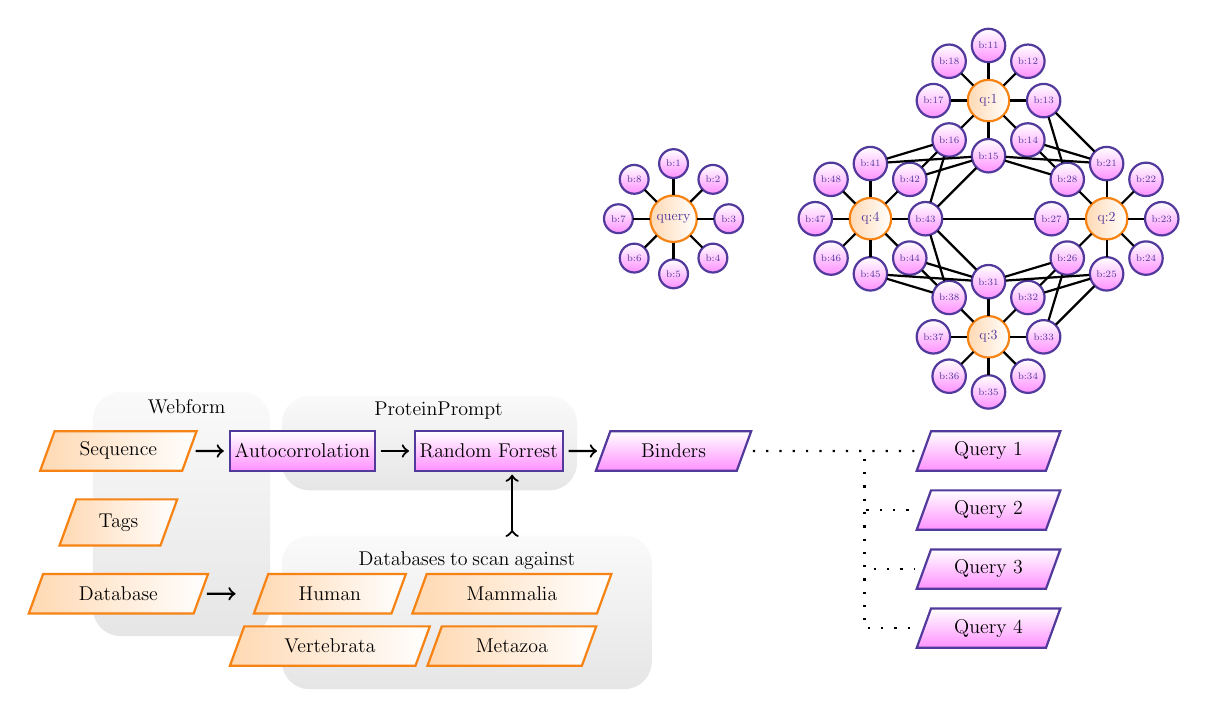
\begin{tikzpicture}[auto,thick, scale=0.5, transform shape,align=center, node distance = 1.5cm]

    \node[queries] (n0) at (-4,0) {query};
    \foreach \k/\l/\j in {1/1/2,-1/1/8,1.4/0/3,-1.4/0/7,1/-1/4,-1/-1/6,0/1.4/1,0/-1.4/5}{
        \node[neighbors] (n\j) at (\k-4,\l) {b:\j};
        %      \path (n\i\j) edge (\i);
        \draw (n\j) -- (n0);
    }
  \foreach \x/\y/\i in {1/0/4,7/0/2,4/3/1,4/-3/3} {
    \node[queries] (\i) at (\x,\y) {q:\i};
    \foreach \k/\l/\j in {1/1/2,-1/1/8,1.4/0/3,-1.4/0/7,1/-1/4,-1/-1/6,0/1.4/1,0/-1.4/5}{
        \node[neighbors] (\i\j) at (\x+\k,\y+\l) {b:\i\j};
        %      \path (n\i\j) edge (\i);
        \draw (\i\j) -- (\i);
    }
  }

  \foreach \i in {5,6}{
    \foreach \j in {1,2,3}{
      \draw (2\i) -- (3\j);
      \draw (1\i) -- (4\j);
    }
  }
  
  \foreach \i in {3,4,5}{
    \foreach \j in {1,8}{
      \draw (4\i) -- (3\j);
      \draw (1\i) -- (2\j);
    }
  }
  
  \draw (43) -- (27);


  

  \node (r1) [res, below of=35] {Query 1};
  \node (r2) [res, below of=r1] {Query 2};
  \node (r3) [res, below of=r2] {Query 3};
  \node (r4) [res, below of=r3] {Query 4};

  \node (webform) [grey, minimum width = 4.5cm, minimum height=6.2cm] at (-16.5cm,-7.5 ) {\parbox[t][5.8cm]{1.7cm}{\Large  Webform}};

  \node (server) [grey, minimum width = 7.5cm, minimum height=2.4cm] at (-10.2cm,-5.7 ) {\parbox[t][2.1cm]{2.8cm}{\Large  ProteinPrompt}};

  \node (result) [res] at (n5 |- r1) {Binders};

  \node (prompt) [process, left=1cm of result] {Random Forrest};

  \node (ac) [process, left=1cm of prompt] {Autocorrolation};

  \node (seq) [io, left=1cm of ac] {Sequence};
  \node (tag) [io, below=0.7 of seq] {Tags};
  \node (db)  [io, below=0.7 of tag] {Database};


  \node (backdb) [grey, minimum width=9.4cm, minimum height=3.9cm] at (-9.25cm,-10cm) {\parbox[t][3.1cm]{5.5cm}{\Large Databases to scan against}};
  
  \node (db1) [io, right=1.5cm of db] {Human};
  \node (db2) [io, right=0.5cm of db1] {Mammalia};
  \node (db3) [io, below=0.3cm of db1] {Vertebrata};
  \node (db4) [io, below=0.3cm of db2] {Metazoa};

  \draw [->, shorten >=2pt, shorten <=2pt] (seq) -- (ac);
  \draw [->, shorten <=2pt, shorten >=9pt] (db) -- (db1);
  \draw [->, shorten >=2pt, shorten <=2pt] (ac) -- (prompt);
  \draw [->, shorten >=2pt, shorten <=2pt] (prompt) -- (result);
  \draw [->, ] (-8.1,-7.9) edge (-8.1,-6.5);

  \draw [loosely dotted, shorten >=3pt, shorten <=3pt] (result) -- (r1);
  \draw [loosely dotted, shorten >=3pt] (0.85,-6.1) |- (r2);
  \draw [loosely dotted, shorten >=3pt] (0.85,-6.1) |- (r3);
  \draw [loosely dotted, shorten >=3pt] (0.85,-6.1) |- (r4);

  
  
\end{tikzpicture}
\end{document}

  \caption{Workflow of the \tool\  server: the user has to provide the query sequence, a tag for later identification, and to select the database in which potential binders are expected. \tool\  converts the sequence first into autocorrelation descriptors prior to calling the random forrest algorithm. The server returns a list of potential binders, sorted by expected binding strength. The website displays the results as a table, that can be filtered by keywords and sorted by several criteria. Additionally, a download link is provided. Having accumulated the lists for several queries, connectivities and thus complex binding networks can be explored. }
\end{figure}

\begin{figure}
%  \include{material/webform}
  \caption{The webform of \tool.
    Required inputs are the sequence and a tag, allowing to locate results.
    Users providing their email will be able to access their results for 2 weeks.
    By default, the query sequence is scanned against the (filtered) human database, containing XX entries.
    Other organisms can be selected in the drop-down.
    (Subject to further development until publication.)}
\end{figure}




\bibliographystyle{naturemag}
\bibliography{ppi_prediction}



\end{document}


